\pattern{Virtual Machine (VM)}
\begin{summary}
    Static description: The {\bf virtual machine} is a middleware between the
    user and physical machine.

    Dynamic description: The {\bf virtual machine} style allows separation
    between user applications with Operating systems. This allows scalability
    and decouples layers so developers can ignore hardware issues.
\end{summary}

\subsubsection{Functional Properties}
\begin{description}
    \item[Multiple Operating Systems] Using a virtual machine
        allows a user to install and use multiple operating system on one
        physical machine. This reduces costs, as users no longer need to
        purchase additional physical machines to run separate operating systems
        and software. This also increases productivity and efficiency since all
        tasks can be performed on a single machine instead of on multiple
        machines.

    \item[Resource Sharing] There is a layer of software between the virtual
        machine and the host called the {\bf hypervisor} that is responsible
        for dynamically allocating resources from the host's memory to the
        virtual machine to allow multiple virtual machines to share
        resources between themselves. This allows a user to transfer files
        between virtual machines and the host (for example, to compile for
        different systems) without the hassle of needing to transfer files
        between machines.
\end{description}

\begin{nfps}
\item[Scalability] Without the need to purchase vast amounts of physical
    hardware to support different OS's, setting up virtual machines is much
    cheaper and less time consuming. New virtual machines can be added or
    expanded upon without having to add additional physical resources.

\item[Maintainability] Due to the nature of virtual machines being pieces of
    software, backups of virtual machines can be made easily as the states of
    these machines can be easily recorded into files. Since the states of
    virtual machines are just files on the host, they can also be easily cloned
    and used on another physical machine.

\item[Security isolation] Virtual machines are designed in such a way to make
    software think it is running in a native operating system on a physical
    machine and that includes viruses and malware. Malware will only run on the
    virtual machines which will have no impact on the host. Since
    backups are easily made, a clean version of the virtual machine can also be
    easily restored.

\item[Negative Efficiency] Virtual machines are often slower than physical
    machine due to indirect access to the host hardware. This means there is
    higher response time.

\item[Negative Efficiency] Virtual machines use more resource due to
    program overheads. For example, some virtual machines allocate disk space
    but it's idle. This lends to waste in disk/memory space since the host
    machine thinks it is in use.

\item[Negative Dependability] When running multiple virtual machines on the
    host OS there could be conflicts which lead to crashes and faults.
\end{nfps}

\begin{center}
    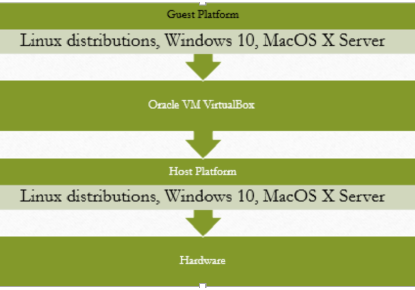
\includegraphics[width=0.4\textwidth]{./virtual-machine}
    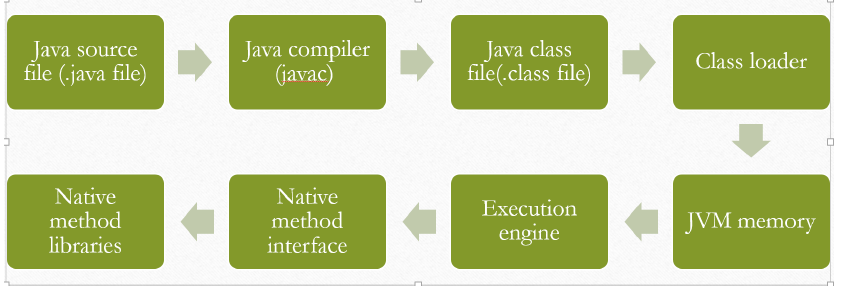
\includegraphics[width=0.4\textwidth]{./virtual-machine2}
\end{center}
